\section{Related Work}
\label{sec:grammars-and-metamodels:Related-Work}

We chose to design and implement a new surface language instead of implementing a design proposed by others.
Section~\ref{sub:grammars-and-metamodels:Surface-languages} describes two existing proposals for surface languages and indicates why we decided not to implement either of them.
There are many alternatives for the languages we used to implement our surface language.
Section~\ref{sub:grammars-and-metamodels:Related-Grammarware} lists a number of alternatives for the grammarware we used and Section~\ref{sub:grammars-and-metamodels:related-Modelware} lists a number of alternatives for the modelware we used.
Section~\ref{sub:grammars-and-metamodels:related-Embedding} describes another approach for integrating textual and graphical modeling languages.


\subsection{Surface Languages}
\label{sub:grammars-and-metamodels:Surface-languages}

Dinh-Trong, Ghosh, and France propose an Action Language based on the syntax of \Java~\cite{JAL}.
We decided not to implement their Action Language because their definition of the language contains a number of primitive types and \Java constructs whose relation to the \UML is not specified.
Other important features of their language are that parameters that serve as input or output of an \Activity and attributes with multiplicity greater than one are not taken into account.

Haustein and Pleumann propose a surface language that is an extension of the \OCL~\cite{Haustein:2004:WRKUMLOMDE,OCLspec}.
They embed \OCL expressions in their language by adding an \Action to the \UML that evaluates an \OCL expression and returns the resulting value.
We took a different approach because we wanted to design and implement a simple alternative for activity diagrams that did not rely on or incorporate other languages.
Incorporating an expression language like the \OCL in our language would introduce a large number of language constructs that have no relation to our primary interest, which is the specification of behavior.


\subsection{Grammarware}
\label{sub:grammars-and-metamodels:Related-Grammarware}

\SDF is based on \SGLR, a scannerless generalized LR parser~\cite{Vis97.thesis}.
As an alternative to using \SDF, \SGLR can be used directly to parse textual representations of models.
However, this requires either manual creation of the parse tables that \SGLR takes as input or generating them from language descriptions formalized using a custom syntax definition formalism.
Since \SGLR can parse arbitrary languages with a context-free syntax and context-free languages are closed under union, multiple syntax definitions can be combined into one without any modifications to the original syntax definitions, as is the case for \SDF.

Other common tools used for parsing, such as \ANTLR, \JavaCC~\cite{JavaCC}, and \YACC~\cite{Joh75.yacc}, can also be used to parse textual representations of models.
They pose more restrictions on the grammars used for the description of the textual representations, however, since the grammars need to be of the LALR or the LL class.

After parsing the textual representations of models, the resulting parse trees have to be transformed.
Besides using special purpose transformation tools, generic programming languages can be used to manipulate the parse trees.
The source transformation language \TXL~\cite{TXL-Cordy} is an example of a special purpose language.
Paige and Radjenovic~\cite{TXLtowards}, and Liang and Dingel~\cite{TXLeval} have experimented with \TXL in the context of model transformation.
Although their research also deals with using grammarware for transformations related to models, it differs from ours because it does not focus on the integration of text-based and metamodel-based languages.

\StrategoXT provides an alternative for \ASFSDF~\cite{BravenboerKVV08}.
It is a language and toolset for program transformation that also uses \SDF for parsing.
It offers programmable rewrite strategies, which allow its users to define the order in which rewrite rules are applied.
In \ASFSDF, the user has no control over the order of application.
In contrast to \ASFSDF, \StrategoXT is not supported by an IDE.

\subsection{Modelware}
\label{sub:grammars-and-metamodels:related-Modelware}

\TCS \cite{TCS} is an alternative for \Xtext.
It is suited for both text-to-model and model-to-text transformations and uses one specification to define the transformations in both directions.
In the case of \TCS, the main constructs are called templates.
These templates are similar to the rules of \Xtext; each template specifies the textual representation of an instance of an element of the metamodel.

\begin{figure}
\centering
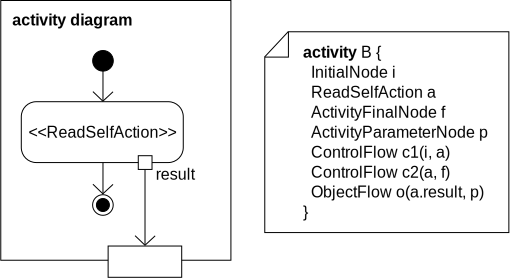
\includegraphics[scale=0.5]{grammars-and-metamodels/figs/mapping-comparison}
\caption{An activity diagram and a straightforward textual equivalent}
\label{fig:grammars-and-metamodels:straightfwd}
\end{figure}

Figure~\ref{fig:grammars-and-metamodels:straightfwd} illustrates how the resulting languages differ from our surface language in case a straightforward mapping, like those offered by \Xtext and \TCS, is used without additional transformations.
The behavior shown in Figure~\ref{fig:grammars-and-metamodels:straightfwd} is equivalent to the behavior shown in Listing~\ref{lst:grammars-and-metamodels:Extracted-SL}.
The description of behavior shown in Figure~\ref{fig:grammars-and-metamodels:straightfwd} is much more wordy than that of Listing~\ref{lst:grammars-and-metamodels:Extracted-SL}, even for such a trivial example.

There are many languages for model transformation, including \QVT~\cite{QVTspec}, ATL~\cite{ATLqvt}, and Epsilon~\cite{conf/icmt/KolovosPP08}.
Since our approach does not rely on any specific properties of \Xtend, each of these transformation languages can replace \Xtend in our implementation.


\subsection{Embedding Textual Modeling into Graphical Modeling}
\label{sub:grammars-and-metamodels:related-Embedding}

Scheidgen's approach for integrating textual and graphical modeling languages~\cite{conf/ECMDA/Scheidgen08} is based on the fact that Eclipse uses the \emph{Model View Controller} pattern~\cite{reenskaug79}.
A mapping from textual notation to metamodel elements is used to generate a model from a textual representation of that model and vice versa.
This custom textual notation and the graphical notations provided by \Eclipse provide independent \emph{Views} for the same \emph{Model}.
The \emph{Controller} is used to modify the underlying model without interfering directly with the other views.
The embedded text editor contained in the implementation of this approach offers syntax highlighting and code completion.
Similar to \Xtext and \TCS, the language describing mappings from textual notation to metamodel elements offers only straightforward mappings, which makes it less flexible than the approach using grammarware. 